\section{Funktionen}

\subsection{Vorhandene User anzeigen}

Startet man das Programm wird gleich die Hauptmaske angezeigt. Auf dieser werden alle Operationen außer das Erstellen von Benutzern ausgeführt. 
Zum Start des Programmes werden alle vorhandenen Benutzer automatisch geladen. Dies ist auf der Grafik \ref{fig:main} zu sehen. Im rechten Teil der Maske exisitert eine ListBox, welche alle vorhandenen User anzeigt. 
Möchte man nach bestimmten Usern selektieren, ist durch das Textfeld über der Liste eine abfrage möglich. Hier spielt Groß- und Kleinschreibung keine Rolle. 
Durch Return (Enter) bestätigt man die eingabe, und es werden nur noch User angezeigt, die auf die Eingabe zutreffen. Will man seine Selektierung rückgängig machen, muss man die Eingabe in das Suchfeld löschen und danach wied er mit Return bestätigen.
Ein Beispiel für das Suchen von Usern ist in Abbildung \ref{fig:user_anzeigen} zu sehen, angezeigt.

\subsubsection{Fehlerbehandlung}

Der einzige Fehler, welcher beim Laden der User auftreten kann, ist dass keine Verbindung zum SAP-System besteht. Ist dies der Fall, wird eine entsprechende Fehlermeldung wie in Abbildung \ref{fig:keine_verbindung} zu sehen.

\begin{figure}[h]
	\begin{center}
		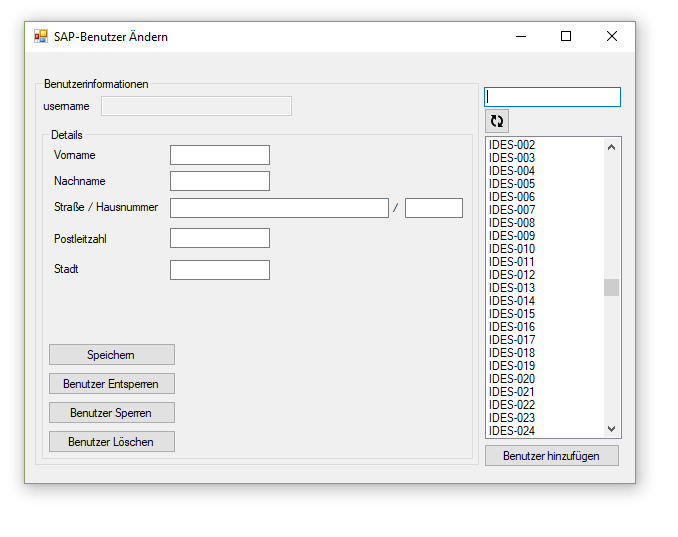
\includegraphics[width=\textwidth]{images/Main.png}
	\end{center}
	\caption{Hauptmaske}
	\label{fig:main}
\end{figure}

\begin{figure}[h]
	\begin{center}
		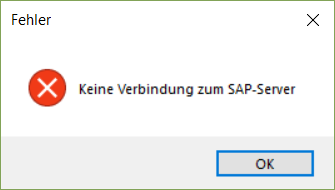
\includegraphics[]{images/Keine_Verbindung.png}
	\end{center}
	\caption{Fehler beim Verbinden zum SAP-System}
	\label{fig:keine_verbindung}
\end{figure}

\subsection{User-Details anzeigen}

Klickt man in der ListBox auf einen User, so werden Details zu diesem geladen. In diesem Programm werden sein Vorname, der Nachname sowie die Anschrift geladen. 
Technisch ist noch vieles Weiteres möglich, was in dieser Arbeit allerdings nicht behandelt wird. Zu sehen ist dies in \ref{fig:user_anzeigen}. 

\begin{figure}[h]
	\begin{center}
		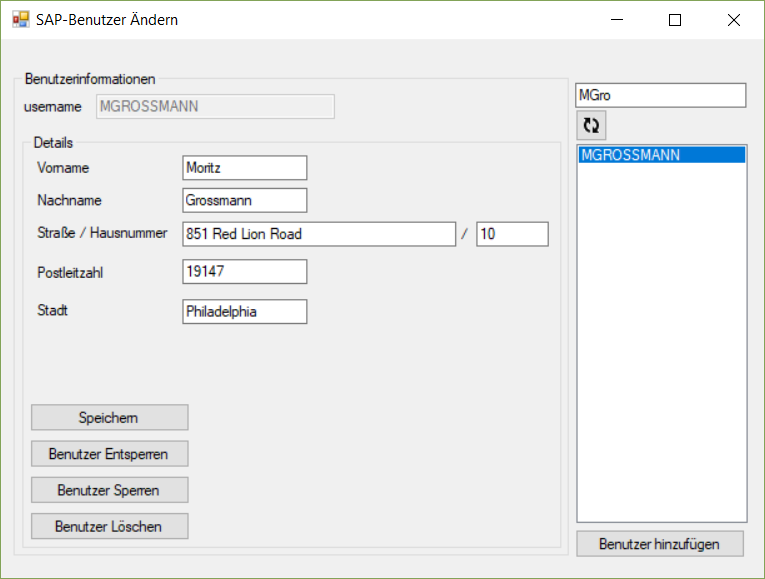
\includegraphics[width=\textwidth]{images/User_Anzeigen.png}
	\end{center}
	\caption{Userdetails anzeigen}
	\label{fig:user_anzeigen}
\end{figure}

\subsection{User erstellen}



\subsection{User editieren}

\subsection{User sperren}

\subsection{User entsperren}

\subsection{User löschen}